\setcounter{chapter}{1} 
\chapter{Theoretical Background} \label{ch:theoretical_back}
% Parametrization (atmospheric modeling), a method of approximating complex processes.
In this thesis I will present motivation, necessary theoretical background and practical implications. 
\\ \\ 
The methods for the data driven approach for parameterization of clouds. It is used as a tool for approximation the complex process of cloud formation. Hopefully this will contribute to the understanding of the physical process which is cloud formation. The data used is a mix of satellite retrievals and reanalysis data. No ancillary information is provided. See sections \ref{sec:era5} to \ref{sec:meteosat} for more detailed descriptions. The numerical methods used in this thesis are described in section \ref{sec:comp_met}. All the code is available on GitHub in the project repository named MS on \href{https://github.com/hannasv/MS}{https://github.com/hannasv/MS}. At this repository you will find everything you need to perform this experiment yourself. Descriptions for downloading data and retrieving the correct licences. Conda envionments listing the python packages and version used to run this code. The project environment is called \textit{sciclouds}. Notebooks for conducting the experiments. Supplementary material for remapping satellite data and land-sea masks are available in a supplementary repository called \textit{MS-suppl}  \href{https://github.com/hannasv/MS-suppl}{https://github.com/hannasv/MS-suppl}.

%\subsection{Cloud feedbacks from convection and fronts} %Cloud, circulation and climate sensitivity article.
\subsection{Parameterizations of clouds}
\textbf{From Tomkins summary}
In order to incorporate the effect of the sub gridscale processes to the climate system one use paramtrizations. Clouds are one of these processes which are usually parametrized. Since this thesis concerns the parametrization of cloud cover. This is the only process which will be discussed. Several other processes are also parameters, like \textbf{give examples}. The simplest form of cloud scheme is if $RH > 100 \rightarrow CLA = 1$ else $CLA = 0$. To achieve a fractional cloud cover one needs a sub gridscale variation in humidity. This could be combined with a sub gridscale of temperature. Over the years reaserchers have tried to draw the distrubutions of these variables from observations and implement them into models. Vitualy all probability density functions, PDF's have been used to model either cloud cover or its dependant variables humidity, temperature and so on.  
\\ \\
Cloud cover is usually a combination of several parametrizations. Its common to have seperate schemes for ice-, liquid clouds and convections.
\\ \\ 
%What is necessary to understand why clouds are Parameterisations. Cite that all climate models are wrong but some are useful.
\subsubsection{Parametrizations of clouds Climate models} \label{sec:climate_models}
Climate models are an important tool for studying the effects of emissions (= forcing) on future climates. The intergovernmental panel of climate change provide assessments report every ~10th year or so, providing a state of the art status update on the current knowledge of climate change. The previous report published was Assesment report 5, AR5 in 2013 and the next report is scheduled to be published in 2021. The ensamble of climate models included in AR5 is \acrfull{cmip5}. \acrshort{cmip6} are now being evaluated, thus there is less published literature. Even though its a bit old, we will mostly focus on the results in AR5. In resent years a lot of effort have been invested in improving the parametrizations of subgridscale processes. Among these clouds contribute with the largest uncertainty, approximately three times as large as other process i.e. relative humidity\textbf{ + another one}. The contributions of the clouds to the short wave component in the radiative budget is the main contributor to the uncertainty. Short wave cloud feedback. 
\\ \\
The computational cost of generating these large ensambles are limiting factor. Simplyfied models in terms of resolution and/ or coplexity is common. 
\\ \\ 
Using idealised experiments they give model spread in \acrfull{ecm}. This describes the \textit{equilibrium change in global and annual mean surface temperature after doubling the $CO_2$ conditions from preindustrial times.}
For \acrshort{cmip5} the \acrshort{ecm} is $2.1^oC$ to $4.7^oC$.The is \textit{very high confidence} that clouds are the primary factor attributing to the wide range. This is not a very big improvement from Hansen et. al. 1984 first estimate of climate sensitivity which was the range $2.0^oC$ to $5.0^oC$. \textbf{explain idealised experiments.} Hansen et al ran their experiments using a coarse resolution of $8^ox10^o$ gridbox (lat x lon) and a doubling of the $CO_2$ concentrations from 315ppm to 630ppm. The \acrshort{cmip5} 

\subsubsection{ERA5} \label{sec:paramERA5}
ERA5 is produced used IFS cycle. This has a new cloud scheme or hydrological cycle. 


\subsubsection{Practical implications} \label{sec:practical_implications}
\textbf{Explain the streength and weakneses of this approach for future implementations. Hva er tatt høyde for ved valg av data og lignende. Kan være nyttig for om folk reproduserer det og skal jobbe videre...}
%  when  using machine learning models as parametrization
One of the obvious downsides of using this approach is the rigid resolution. 
Climate models provide data in a wide range of different of spatiotemporal resolutions. 
\\ \\ 
Before implementing this model it would need to be retrained on the resolution of the climate model under development. Which includes both remapping the data set and retraining the model. This is a time consuming process involving finding a new set of hyperparameters suitable for the new resolution. Once trained machine learning models provide fast results even for complex parametrizations which is what makes them suitable. \\ \\ global view of satellites can be useful. 

\section{Data set and Methods}
\subsection{ERA5} \label{sec:era5}
ERA5 is the latest in the series of reanalysis produced by \acrfull{ecmwf}. Re-analysis is as close to observations as one can get coherent in space and time. Sometimes people forget that it is assimilated against observations not observations. Data assimilation takes in observations and tries to make a accurate estimate of the state of the system. In climate (\textbf{atmospheric?}) science this includes both ground based, ships, \textbf{buyes/bøyer?}, airplanes and satellites. The analysis is produced in the operational system, making it available within five days of real time. ERA5 is based on the Integrated Forecasting System, IFS cycle 4lr2. The data is available in $0.25^o$ degree and hourly resolution. Its an important product in the continuous climate monitoring.  
\\ \\
The all sky radiance's from \acrfull{msg} in the period 2003-2012 is included in the assimilation's. This is the sate satellite as I gather the cloud masks.
\\ \\ 
Reanalyses data is often mistakenly referred to as observations. This is the theme of the essay in \textit{Reanalysis and Observations - What the difference?} published in \acrfull{bams} 2015. They conclude with that they are not to different. Both involve inference (theory based calculations) and re-analysis relies on forecast and observations does not. This is not a significant difference as long as the forecast is sufficiently accurate. Its important to be aware of that the uncertainty of the reanalysis is less well known than for observations. This makes it harder to judge appropriate use of the reanalysis. 

\textbf{Summaries their conclusions. }  
 

\subsection{METEOSAT Second Generation - SEVRI} \label{sec:meteosat}
The highest resolved satellite measurements come from geostationary meteorological weather satellites. Polar orbiting satellites usually provide daily resolution. (STUBENAU). There is also a wide range of viewing angles. The orbit of MODIS makes sure it has the exact same viewing angle every 16th day. The angle attributes so small differences in detected cloud mask. This also occurs when the standby satellite of METEOSAT 

The second generation satellite consist of METEOSAT 8 to 11. The MSG system provides a two satellite system. The operational satellite at a nadir point of $0^o$ latitude. \textbf{ref. introduction MSG2} and the standby satellite. Sometimes both satellites gather data at the same time. Then the standby-satellite grid is rectified to a a grid of the operational one (Personal correspondence with the help-desk). In these images it becomes evident that viewing angle affects the retrievals. When this duplication occurs, the operational satellite is chosen. The temporal resolution of 15min and the nadir pixel size is 3km (Taravat, 2015). The sensor SEVERI har 12 channels. One broadband visible channel, three solar channels (0.6, 0.8 and 1.6 $\mu m$) and 8 thermal infrared channels (3.9, 6.2, 7.3, 8.7, 9.7, 10.8, 12.0 and 13.4 $\mu m$). (Taravat, 2015 - should probably find the source online on EUMATSAT web pages).
\\ \\ 
\textbf{More practical implications}. This one has two partners covering the Indian and Pacific ocean. Together they give almost a global view, discarding the poles. This will be useful if this trail run is successful.  \textbf{programming language. how to best implement them in }
%You may calculate the difference of the measurements, e.g. for channels VIS0.6, IR3.9 and IR10.8 between the two satellites. This will give an estimate how large the measurements differ and as a consequence the products (e.g. cloud mask) will be different.\textbf{also personal corespondance.}

\subsection{EUMETSAT Cloud Mask} \label{sec:cloud_mask}
The EUMETSAT cloud mask, CLM relies on the fact that clouds are colder and more reflective than the surface. They also reclassify isolated pixel. The data is available on Earth Observation Portal on EUMETSATS web pages. CLM consist of four classes, zero - clear sky over ocean, one which is clear sky over land, 2 denotes cloudy and 3 is outer space/off earth disk/no data. These classes are derived from almost all channels except (X) \textbf{cite article 10 in Tavarat, 2015}.

The cloud mask is distributed in GRIB-format (no coordinates) and NC-format (coordinates). Due to spatial limitations (Since all files have the same coordinates) one NC-files is downloaded for the coordinates and the rest of the data has been downloaded in GRIB-format. Some retrievals are excluded because of high uncertainty in the measurements this creates gaps in the data set. 

\subsection{MODIS - If you include comparisons to verify own sat elite computations.} \label{sec:modis}
\textbf{Something on modis.}
% Please add the following required packages to your document preamble:
% \usepackage{multirow}



\subsection{Thoughts when choosing the data set of satellite images}
Choose the finest temporal resolution possible. The average lifetime of a cloud is an hour. Since this is a proof of study is seems reasonable to choose the finest resolution available. Here this is METEOSAT.
In future work it would be interesting to asses how data driven parametrization compare to the existing parametrizaions available in the state of the art climate models. Here both the temporal and spatial resolution is a lot coarser. Other data sets could be considered. The masks in other data sets are computed based on more channels than in METEOSAT but the temporal resolution is a lot worse. 

\subsection{European Cloud Cover}
\textit{Add somewhere from personal correspondence the gaps are caused by: We regret to inform you that unfortunately we cannot process your orders 1368572 and 1368598. The data was corrupted prior archiving to tape and this data file cannot be recovered. }
For the purpose of this thesis a new data set was built. The clouds in ERA5 is models according to the descriptions in \ref{sec:paramERA5} so I had to look elsewhere for a suitable \textit{true value} to regress the meteorological variables against. Keep in min the hourly temporal resolution and $0.25^o$ spatial resolution in ERA5. Most satellite products move in polar orbits and finer resolution than daily is rare. Vertically resolved data was also unnecessary. \textbf{cite Calipso and Modis}. This guided me in the direction of the satellites in geostationary orbit. The only geostationary satellite covering the east Atlantic is the 0 degree \acrfull{msg} satellite. With the high temporal resolution of 15min and a fixed grid is seemed like a reasonable choice. %This is beneficial when learning from data. 
Preserving the resolution available from ERA5, remapping the cloud mask to cloud fractions also know as cloud amount. \textit{\acrshort{ecc} comprises of five variables collected from two sources; ERA5 and EUMETSAT}The final product consist of the variables temperature, pressure, cloud amount, specific and relative humidity. Hourly data on a $0.25^o$ resolution in the period \textbf{put in first date} to \textbf{last date}. 
For this project the geographical domain has been restricted latitude $\in[30,50]$ and longitude $\in [-15, 25]$. This becomes 80x160 pixels for each time step. As always when working with observations, data is missing. Since the individual pixels are remapped to fractions by using the area weighted mean, NaN's are not a issue. For sometimes no cloud masks are available. Then the closest time step available within the previous and trailing 45 minutes are chosen. Other gaps are documented in \textbf{X}. 
\\ \\
The original data is described in table \ref{tab:dataset_summary} and the finished product is described in the \ref{tab:ecc}. The demanding process of remapping the mask to fraction is presented in section \ref{sec:remapping}
% more detailed description on what ERA5 is and how it is produced is described in section \ref{sec:era5}. 
% As table \ref{tab:variables} shows the data set comprises of five variables collected from two sources; ERA5 and EUMETSAT. Temperature, surface pressure, specific and relative humidity is collected from ERA5. More information about this is available in section \ref{sec:era5}.
Fractional cloud cover is computed from the cloud mask product retrieved by the second generations METEOSAT satellites. You can read more about this data in section \ref{sec:meteosat}. For simplicity we will refer to this dataset as European Cloud Cover Dataset, ECC from now on. 
\\ \\ 
%This includes METEOSAT 8, 9, 10 and 11.
The mapping from the curve-linear grid of the geostationary satellite to the uniform grid of era5 is quite technical and is described in section \ref{sec:regridding}. The cloud amount of a pixel is the sum of the area weighted cloud mask contributing to a cell.

\begin{table}[]
\begin{tabular}{|c|c|c|c|c|c|}
\hline
\textbf{Source}                & \multicolumn{1}{c|}{\textbf{Type}}               & \textbf{Variables}         & \textbf{Projection}                    & \textbf{Availability}          & \textbf{Licence}                                                                                                                   \\ \hline
\multirow{4}{*}{ERA5} & \multirow{2}{*}{Surface}                & 2m Temperature    & \multirow{4}{*}{Uniform grid} & \multirow{4}{*}{1979 - dd.} & \multirow{4}{*}{\begin{tabular}[c]{@{}c@{}}Need user on \\ Copernicus Data Store. \\ Available for everyone.\end{tabular}} \\
                      &                                         & Surface pressure  &                               &                             &                                                                                                                            \\
                      & \multirow{2}{*}{1000 hPa}               & Relative Humidity &                               &                             &                                                                                                                            \\
                      &                                         & Specific Humidity &                               &                             &                                                                                                                            \\ \hline
MSG                   & \multicolumn{1}{c|}{Satellite retrival} & Cloud Mask        & Curvelineaer grid             & 2004-dd.                    & \begin{tabular}[c]{@{}c@{}}Higher than 3hourly \\ resolution requires a \\ reaserchers liscence.\end{tabular}              \\ \hline
\end{tabular}
\caption{Data description on the data present in the dataset ECC (European Cloud Cover). \textbf{Add projection as a column, Availability for download and the period of data.}}
\label{tab:dataset_summary}
\end{table}

\begin{figure}[h]
    \centering
    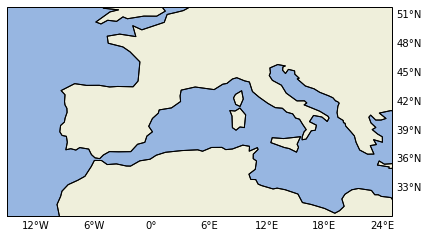
\includegraphics[scale = 0.7]{Domain.png}
    \caption{Map showing the domain. The region cover southern Europe and northern Africa. The coordinate system is Plate Caree, which is the same as ECC. The image have been generated using the python package cartopy ref? \textbf{new figure with correct range and some vegetation or topography on  }}
    \label{fig:map}
\end{figure}

\begin{figure}[h]
    \centering
    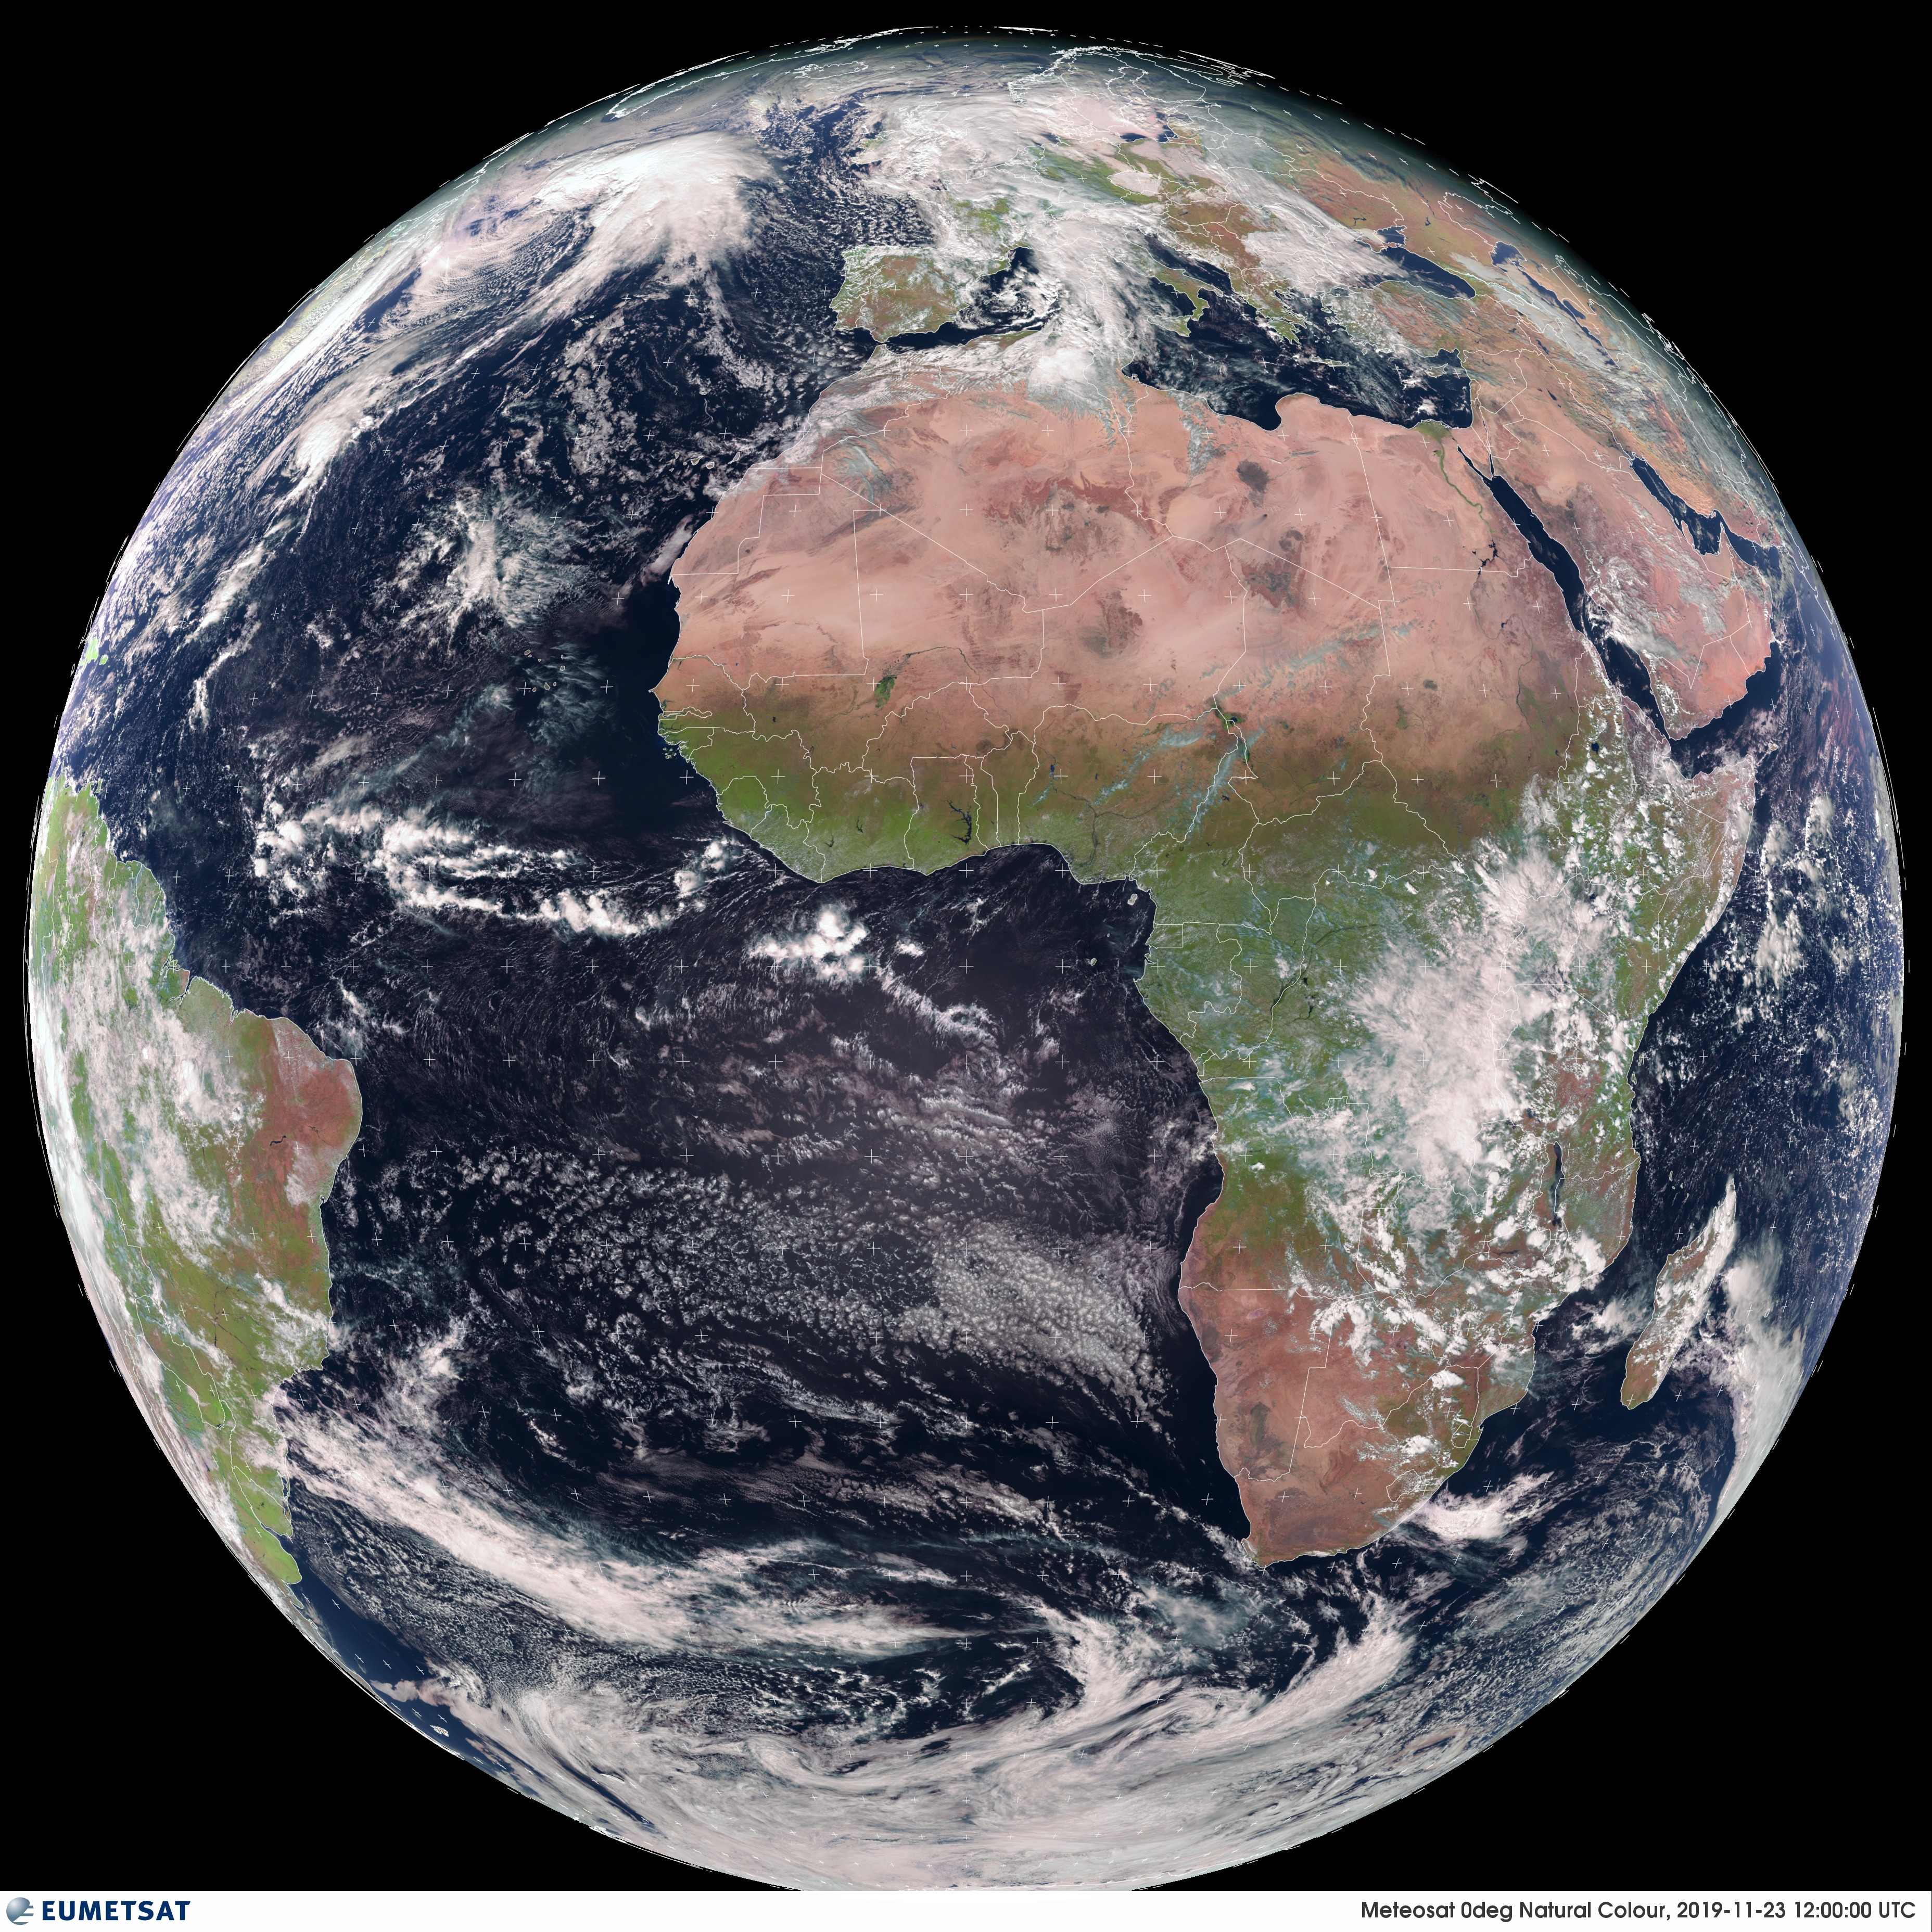
\includegraphics[scale=0.11]{MET10_RGBNatColourEnhncd_FullResolution_20191123120000.jpg}
    \caption{The view of the earth from \acrshort{msg}. The picture is dated noon on the 11 November 2019. \textbf{Cite EUMETSAT}. By studying the patterns it becomes evident that clouds are influenced by the circulations. }
    \label{fig:sat_view}
\end{figure}

%%%%%%%%%%%%%%%%%%%%%%%%%%%%%%%%%%%%%%%%%%%%%%%%%%%%
\subsubsection{Physical basis of variable decision}
The variables have been chosen based on availability, \textit{uncertainty/ quality} and their contribution to the physical processes. As mentioned in the introduction clouds require a aerosol and sufficient supersaturation.\textit{ However up-draft velocities and aerosols (especially type) is difficult to impossible to know?} \textbf{kilde?} I hypothesis that some of this information is present in temperature, humidifies and surface pressure in space and time and thus the cloud cover can be inferred patterns of these variables. Except for rural areas there is usually \acrshort{cnn} and/or \acrshort{inp} present. \textbf{lov å si kilde!}

\paragraph{Temperature}\mbox{}\\ % Need this line otherwise its 
The temperature is the two meter temperature produced by ERA5. For simplicity this will be referred to as temperature from now on. High temperature is related to convection. The air close to the surface gets heated, this reduces the density and starts the process of rising air masses. As the air rises it cools as a consequence of the work that has been done to the surrounding because of expansion. The temperature could also be a seasonal proxy. 

\paragraph{Humidity} \mbox{}\\
Both specific and relative humidity is included as features. Conditions where relative humidity exceeds 100\% are called supersaturated. Intuitively this should be a good predictor. However since the the clouds don't form at the surface its not clear if specific humidity is a better predictor. Specific humidity is the actual amount of vapour in the atmosphere in units of \textbf{kg/kg?}. \textit{Trude: Can I say that the rate of evaporation at the surface is proporsjonale to the humidity?} To some extent these variables are temperature dependant. Warm air can retain more vapour than cold air. Which is the main reason from precipitation. 
\\ \\
Let humidity be a collective term for both humidity's. The data is gathered from the model level closest to the surface. Which is at a height of 1000hPa. 
\\ \\ 
In order to form a cloud you need the air to exceed a saturation with respect to water or ice. This can with the presence of cloud condensation nuclei/ ice nuclei particles start the cloud formation processes.  On the other hand specific humidity is the actual amount of water vapour present in the atmosphere. 

\paragraph{Surface Pressure}\mbox{}\\ % ikke samme linjeavstand
Due to the earth geometry and the angle of rotation there is a energy surplus at the equator. Winds transport some of this heat pole ward. Geostrophic winds are the large scale balance between the Coriolis force and the pressure gradients. This wind flows parallel to the isobars, lines of constant pressure. Any factor that generates a pressure gradient can create disruptions in the wind pattern's. Topography for instance. For convenience surface pressure will be referred to as pressure in this thesis. \textbf{Don't think including the equation from geostrophic balance improved this section.}
%%%%%%%%%%%%%%%%%%%%%%%%%%%%%%%%%%%%%%%%%%%%%%%%%%%%%%%%%%%%%%%%%%

\subsubsection{Computing cloud fractions} \label{sec:remapping}
The cloud fractions in \acrshort{ecc} is the area weighted cloud masks from \acrshort{msg}. The masks in \acrshort{msg} referred to as clear (0) or cloudy (1).
If there is a NaN present, this pixel is simply excluded. Calculation wise this has the same affect as a clear pixel. \textbf{Should this be updated to remove the area of the cloudy pixel.} 
\\ \\
The METEOSAT cloud mask provided in NetCDF-format contains the coordinate information. Since the coordinate system is constant only one NetCDF files are downloaded.The surface area of a square on a sphere can be computed by solving the integral in \eqref{eq:sphere_integral}. This is the result in \eqref{eq:sphere_finish}. Since the netCDF-files only contain latitude and longitude informa

Before using this formula approximations of the extent of the cell needs to be made.
    
Calculating the area based on a curve-linear grid that only contain information about latitude and longitude involves some simplifications. From \eqref{eq:sphere_finish} 

, which can be rewritten into equation \eqref{eq:sphere_finish}. The latter one is used for implementations. Here R denotes the distance to earth centre, $\theta$ the latitude and $\phi$ the longitude. Approximation of $d\phi$ and $d\theta$ have been done based on the two-dimensional fields of latitude and longitude values according to equations \eqref{eq:app_lon} and  \eqref{eq:app_lat}.

%I have tried to keep these to a minimum and believe that they don't add more uncertainty. 
The visual comparison between raw satellite images and cloud amount seem to agree. The cloud fractional distribution also retain the same shape as ERA5 and MODIS 6.1 terra in the period from 2004 to 2018. 
\\ \\
\textbf{Update equation to use a upside down delta.}
\begin{equation} \label{eq:sphere_integral}
    A = -R^2\int_{ \theta - \delta \theta }^{\theta + \delta \theta} \int_{ \phi - \delta \phi }^{\phi + \delta \phi} cos\left( \theta' \right) d\phi' d\theta'
\end{equation} 

\begin{equation} \label{eq:sphere_finish}
    A \left( \theta, \phi, \delta \theta, \delta \phi   \right)= 2R^2 \left( sin\left( \theta + \delta \theta  \right) - sin\left(  \theta - \delta \theta  \right) \right) \delta \phi
\end{equation} 

The latitude and the extend of the pixel is terms in this equation. The extent of a pixel can also be interpreted as the \textbf{what.} The changes on longitude at a certain pixel is the the average distance to neighbouring points.

\begin{equation} \label{eq:app_lon}
    \delta \phi_{i,j} = \left| \frac{\phi_{i+1,j} - \phi_{i-1, j}}{4} \right|
\end{equation}

\begin{equation} \label{eq:app_lat}
    \delta \theta_{i,j} = \left| \frac{\theta_{i,j+1} - \theta_{i, j-1}}{4} \right|
\end{equation}

The latitude, longitude information is retrieved from the product of the satellite images. In order to keep the data storage to a minimum most files are download in grib-format. All satellite images from the 0 degree service are given with the same coordinates. This became evident from conversation with the help desk. 
\begin{figure}[h]
    \centering
    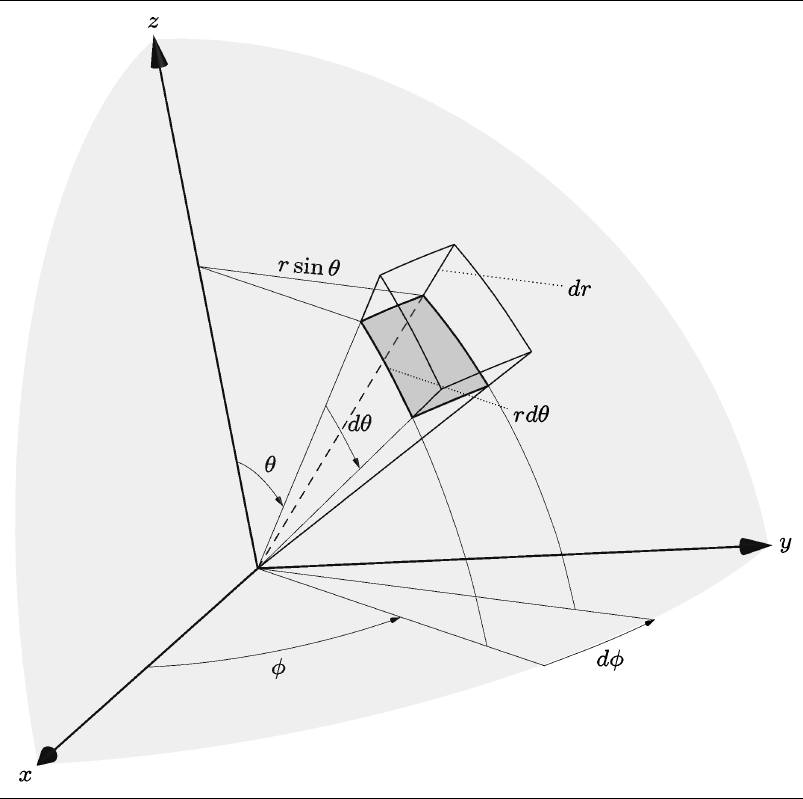
\includegraphics[scale = 0.6]{coordinates.png}
    \caption{Credit, https://tex.stackexchange.com/questions/159445/draw-in-cylindrical-and-spherical-coordinates}
    \label{fig:coords}
\end{figure}

\\ \\
The cloud cover will be referred to as cloud amount, fraction or simply the clouds.
%%%%%%%%%%%%%%%%%%%%%%%%%%%%%%%%%%%%%%%%%%%%%%%%%%%%%%%%%%%%%
\subsubsection{Licences and Downloading Data}
Scripts for downloading the ERA5 data used in this thesis is available in the project GitHub on \href{https://github.com/hannasv/MS/tree/metos/downloading_RA}{https://github.com/hannasv/MS/tree/metos/downloading_RA}. However you will need to create a CDS-user. I suggest you follow the instructions on ECMWF homepages on \textit{how to download ERA5}. 
There are no scripts available for downloading METEOSAT data this is done using satellite retrievals at EUMETSATs Earth Observation Portal. Its freely available in hourly resolution. Scientist can apply for increased resolution up to 15min. You choose the cloud mask product in grb-format. By running \textbf{X - legg inn filnavn} you can remap your own files.
%%%%%%%%%%%%%%%%%%%%%%%%%%%%%%%%%%%%%%%%%%%%%%%%%%%%%%%%%%%%%%%%%%
\section{Computational Methods  - Introduction to machine learning} \label{sec:comp_met}
\subsection{Talk about machine learning in broad terms - then rewrite this to an introduction to chapter}
Machine learning consist of three subcategories supervised-, unsupervised- and reinforcement learning. Supervised learning is the part of machine learning concerned with learning the relation between input data, x and labelled data y. 
\\ \\
In this section I will explain the computational methods used for generating the numerical experiments conducted in this thesis. Starting with the the performance metrics used to evaluate the models. Followed by the auto regressive model and recurrent neural networks. For recurrent nets I will start by explaining the simple feed forward network building up to the more complex recurrent networks. This network is also known as convolution long short-term memory network.
\subsection{machine learning types and what they are useful for}
\textit{designs that utilise their learning. }
\subsection{Supervised learning - Regression}
Present the general idea in a interesting way.

\subsubsection{Autoregressive models} \label{sec:ARmodels}
The autoregressive model is regression method where you allow the state at previous time to be a predictor. As you can see from \eqref{eq:auto-regressive} removing the time dependency leaves the expression of ordinary linear squares, OLS regression. \textbf{Kilde}

\begin{equation} \label{eq:AR}
    \hat{Y_n} = \hat{\beta_0} + \sum_{j=1}^p X_j\hat{\beta_j} + \sum_{i = 1}^{n_{ts}} Y_{n-i}\hat{\beta_{p+i}}
\end{equation}

\textit{include gradient descent here}

\subsection{Neural network}
Introduction. 
\subsubsection{The Perceptron}
\begin{enumerate}
    \item the perceptron 
    \item draw link to one layer nn when you have 1 layer 
    \item feedforward and backprop in perceptron (includes activation and activation functions.)
    \item Mulitple layers here or in its own subsubsection?
\end{enumerate}

\subsubsection{Muliple layers - Deeper networks}

\subsubsection{Convolutional Neural Networks}

\subsubsection{Convolutional LSTM}
\label{sec:conv_lstm}
Key equations in convolutional LSTM is listed in equation (\ref{eq:CLSTM1_input_gate}) - (\ref{eq:CLSTM5_hidden_state}). Here $\circ$ denoted the Hademand product, which is a component wise multiplication, and * is convolution. 

\begin{equation} \label{eq:CLSTM1_input_gate}
    i_t = \sigma \left( W_{xi}*x_t + W_{hi}*H_{t-1} + W_{ci}\circ C_{t-1}+b_i \right) 
\end{equation}

\begin{equation} \label{eq:CLSTM2_forget_gate}
        f_t = \sigma \left( W_{xf}*x_t + W_{hf}*H_{t-1} + W_{cf}\circ C_{t-1}+b_f \right) 
\end{equation}

\begin{equation} \label{eq:CLSTM3_cellstate}
        C_t = f_t \circ C_{t-1} +i_t\circ tanh\left( W_{xc}*X_t + W_{hc}*H_{t-1} + b_c \right)
\end{equation}

\begin{equation} \label{eq:CLSTM4_output_gate}
        o_t = \sigma \left( W_{xo}*X_t + W_{ho}*H_{t-1} + W_{co}\circ C_{t}+b_o \right)
\end{equation}

\begin{equation} \label{eq:CLSTM5_hidden_state}
        H_t = o_t \circ tanh \left( C_t \right)
\end{equation}

\paragraph{Learning algorithmns - optimizen (implementation of sequence length)} \mbox{}\\
Describe the following
\begin{enumerate}
    \item Loss, cost, performance metric? epoch batch
\end{enumerate}

From Chollet book s. 11 \textit{the fundamental trick in deep learning is to use this score (result from performance metric) as a feedback signal to adjust the value of the weights a little, in a direction that will lower the loss score for the current example. } The adjustment is the job of the optimizer, which implements backpropagation algorithmn which is the sentral learning algoritmn.
\textbf{Explain this in words.}



\paragraph{Automatic optimisation}
Keras-tuner .
\textbf{Explain all the params you tune. Might be beneficially with a figure. See Rune's MS-thesis.}




\section{OLD }

\subsection{Performance metrics}  \label{sec:perf_metrics}
In order to acquire a certain skill you need a measure determining how close you are. 

\begin{equation} \label{eq:mse}
    MSE(\hat{y},\hat{\tilde{y}}) = \frac{1}{n} \sum_{i=0}^{n-1}(y_i-\tilde{y}_i)^2
\end{equation} 

\begin{equation} \label{eq:ase}
    ASE(\hat{y},\hat{\tilde{y}}) =  \sum_{i=0}^{n-1}(y_i-\tilde{y}_i)^2
\end{equation} 

\begin{equation} \label{eq:r2}
    R^2(\hat{y}, \tilde{\hat{y}}) = 1 - \frac{\sum_{i=0}^{n - 1} (y_i - \tilde{y}_i)^2}{\sum_{i=0}^{n - 1} (y_i - \bar{y})^2}
\end{equation} 
where mean value of $\hat{y}$ is defined as $\bar{y} =  \frac{1}{n} \sum_{i=0}^{n - 1} y_i$. 

\section{Future work}
\begin{enumerate}
    \item Describe how to make parametrization to implement in CMIP6.
    \item Programming language in climate models vs python.
\end{enumerate}

\section{Good phases}
\begin{itemize}
    \item  In its most simple form, the diffusion equation is given by
    \item By using a finer grid one can usually get better approximations
    \item The comparison will focus on computational time and accuracy.
    \item This was chosen after
studying the development of the loss function as a function of number of iterations
    \item and is mandatory in
more advanced architectures(e.g. residual nets) where a constant spatial
dimension is demanded.
    \item a list of examples and so forth.
    \item (I will reference to source code/project part where relevant!)
    \item out of sample precision.
    \item Learn how to create plots with a zoomed in view.
    \item sufficiently large
    \item Viktig poeng. \textit{However, both academic
researchers and practitioners alike acknowledge the
need to make tests on the actual data set that is
subject of interest, as well as dedicating time and
resources to tune hyperparameters}
    \item methods for tabular data vs images
    \item I have opted to use
    \item We have also modified our own code for a dense feed forward neural
network produced for Project 2, see

\end{itemize}





